\documentclass[12pt]{article}
\usepackage{amsmath,amssymb}
\usepackage[margin=1in]{geometry}
\usepackage{tikz}
\usetikzlibrary{
    arrows.meta,
    calc,
    angles,
    quotes,
    decorations.pathmorphing
}
\usepackage[american]{circuitikz}


\begin{document}

\begin{enumerate}

\item A uniform solid sphere of mass \(M\) and radius \(R\) rolls without slipping from height \(h\) down a rough incline and enters a smooth horizontal surface where it compresses a light spring of constant \(k\). During compression, static friction is just sufficient to maintain rolling and becomes zero exactly at maximum compression. Using coupled translational–rotational dynamics and the condition that angular acceleration vanishes at extreme compression, determine the maximum compression \(x\).\\

% Diagram for Question 1
\begin{center}
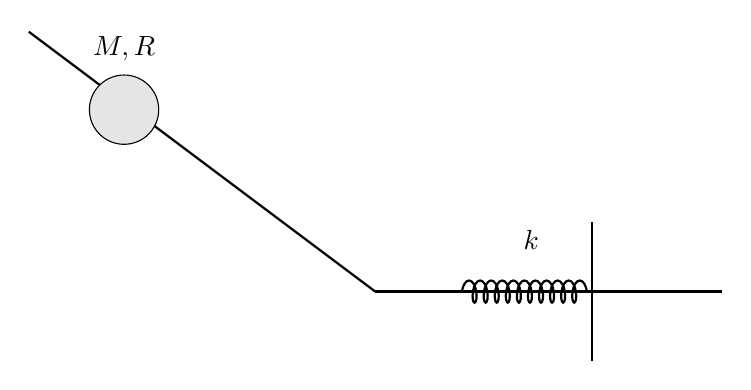
\begin{tikzpicture}[scale=1.1]

% Incline
\draw[thick] (0,3) -- (4,0);
\draw (1.2,2.2) node[left] {$h$};

% Sphere on incline
\draw[fill=gray!20] (1.1,2.1) circle (0.4);

% Ground
\draw[thick] (4,0) -- (8,0);

% Spring
\draw[thick,decorate,decoration={coil,aspect=0.4,segment length=4pt,amplitude=4pt}] (5,0) -- (6.5,0);

% Wall
\draw[thick] (6.5,-0.8) -- (6.5,0.8);

% Labels
\node at (1.1,2.8) {$M,R$};
\node at (5.8,0.6) {$k$};

\end{tikzpicture}
\end{center}

A) \(\sqrt{\dfrac{10Mgh}{7k}}\)\\

B) \(\sqrt{\dfrac{5Mgh}{7k}}\)\\

C) \(\sqrt{\dfrac{10Mgh}{9k}}\)\\

D) \(\sqrt{\dfrac{2Mgh}{k}}\)

\item A uniform rod of length \(L\) and mass \(M\) is hinged at one end and released from horizontal position; the hinge exerts a constant frictional torque \(\tau\) opposing motion. Using rotational work–energy relation about the hinge and accounting for gravitational torque varying with angle, determine the minimum value of \(\tau\) such that the rod just reaches the vertical position with zero angular speed.\\

% Diagram for Question 2
\begin{center}
\begin{tikzpicture}[scale=1.2]

% Hinge
\fill (0,0) circle (2pt);

% Rod
\draw[thick] (0,0) -- (30:3);

% Vertical reference
\draw[dashed] (0,0) -- (90:3);

% Angle (from vertical to rod)
\draw (0,0) arc (90:30:1);

\node at (60:1.2) {$\theta$};
\node at (30:2.2) {$L,M$};

\end{tikzpicture}
\end{center}

A) \(\dfrac{MgL}{2\pi}\)\\

B) \(\dfrac{MgL}{\pi}\)\\

C) \(\dfrac{MgL}{4}\)\\

D) \(\dfrac{MgL}{2}\)

\item A bead of mass \(m\) moves without friction on a circular wire of radius \(R\), the wire rotating with constant angular speed \(\omega\) about a vertical diameter. In the rotating frame the effective potential is \(U=-mgR\cos\theta-\frac{1}{2}m\omega^2R^2\sin^2\theta\); non-trivial equilibrium exists when \(\cos\theta=\dfrac{g}{\omega^2R}\). By expanding the effective potential about this equilibrium up to quadratic order, determine the angular frequency of small oscillations about the stable position.\\

% Diagram for Question 3
\begin{center}
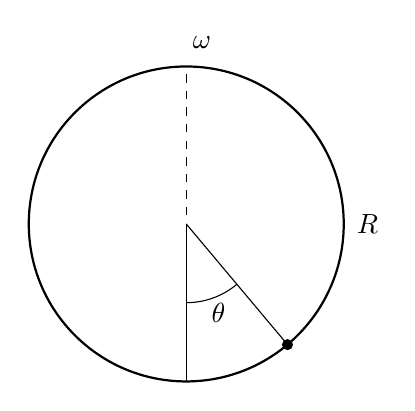
\begin{tikzpicture}[scale=1]

% Circle
\draw[thick] (0,0) circle (2);

% Vertical diameter (axis of rotation)
\draw[dashed] (0,-2) -- (0,2);

% Bead at 40 degrees from downward vertical
\fill (-50:2) circle (2pt);

% Angle theta (measured from downward vertical)
\draw (0,0) -- (-50:2);
\draw (0,0) -- (270:2);
\draw (0,-1) arc (-90:-50:1);
\node at (-70:1.2) {$\theta$};

% Labels
\node at (2.3,0) {$R$};
\node at (0.2,2.3) {$\omega$};

\end{tikzpicture}
\end{center}

A) \(\sqrt{\omega^2-\dfrac{g^2}{\omega^2R^2}}\)\\

B) \(\sqrt{\omega^2-\dfrac{g}{R}}\)\\

C) \(\sqrt{\dfrac{g}{R}-\omega^2}\)\\

D) \(\sqrt{\omega^2+\dfrac{g}{R}}\)

\item Two blocks of masses \(m\) and \(2m\) are connected by a light spring of constant \(k\) on a smooth horizontal surface and initially at rest with spring unstretched. A horizontal impulse gives velocity \(v_0\) to the lighter block while simultaneously giving the heavier block velocity \(-\dfrac{v_0}{2}\). Using conservation of total momentum and energy decomposition into center-of-mass and internal motion, determine the maximum extension of the spring.\\

% Diagram for Question 4
\begin{center}
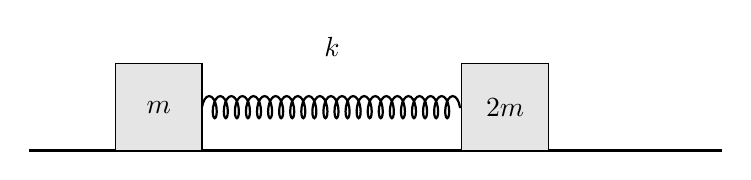
\begin{tikzpicture}[scale=1.1]

% Ground
\draw[thick] (0,0) -- (8,0);

% Left block
\draw[fill=gray!20] (1,0) rectangle (2,1);
\node at (1.5,0.5) {$m$};

% Right block
\draw[fill=gray!20] (5,0) rectangle (6,1);
\node at (5.5,0.5) {$2m$};

% Spring
\draw[thick,decorate,decoration={coil,aspect=0.4,segment length=4pt,amplitude=4pt}] (2,0.5) -- (5,0.5);

% Label
\node at (3.5,1.2) {$k$};

\end{tikzpicture}
\end{center}

A) \(\dfrac{mv_0^2}{k}\)\\

B) \(\dfrac{mv_0^2}{2k}\)\\

C) \(\dfrac{3mv_0^2}{4k}\)\\

D) \(\dfrac{mv_0^2}{3k}\)

\item A particle is projected radially outward from Earth’s surface with speed \(v=\alpha v_{esc}\), where \(0<\alpha<1\). Using conservation of total mechanical energy in gravitational field \(-\dfrac{GMm}{r}\), determine the time taken to reach maximum distance \(r_{max}\) expressed in terms of \(R\), \(g\), and \(\alpha\).\\



A) \(\dfrac{R}{\sqrt{gR}}\dfrac{\alpha}{1-\alpha^2}\)\\

B) \(\dfrac{R}{\sqrt{gR}}\dfrac{\alpha}{\sqrt{1-\alpha^2}}\)\\

C) \(\dfrac{R}{\sqrt{gR}}\dfrac{\alpha}{(1-\alpha^2)^{3/2}}\)\\

D) \(\dfrac{R}{\sqrt{gR}}\dfrac{1}{1-\alpha^2}\)

\item A composite wire consists of two equal lengths joined in series with identical cross-sectional area \(A\) and Young’s moduli \(Y\) and \(2Y\). The wire is stretched by force \(F\), and simultaneously temperature rises so that free thermal expansion would be \(\Delta L=\beta L\) for each segment, but total length is kept fixed. Using compatibility of strain and stress equilibrium, determine the ratio of elastic energies stored in the two segments.\\

A) \(2:1\)\\

B) \(1:2\)\\

C) \(4:1\)\\

D) \(1:1\)

\item A cylindrical vessel of radius \(R\) is filled with liquid of density \(\rho\) and rotates with angular speed \(\omega\); the free surface forms a paraboloid while total volume remains constant. Using conservation of volume and integrating gravitational potential energy over the liquid mass, determine the increase in potential energy compared to the non-rotating state.\\

% Diagram for Question 7
\begin{center}
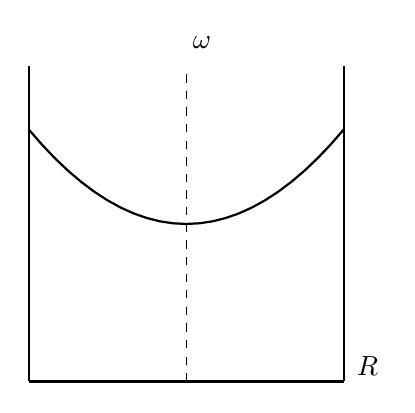
\begin{tikzpicture}[scale=1]

% Cylinder walls
\draw[thick] (0,0) -- (0,4);
\draw[thick] (4,0) -- (4,4);

% Bottom
\draw[thick] (0,0) -- (4,0);

% Parabolic surface
\draw[thick] plot [domain=0:4] (\x,{0.3*(\x-2)^2 + 2});

% Axis
\draw[dashed] (2,0) -- (2,4);

% Labels
\node at (4.3,0.2) {$R$};
\node at (2.2,4.3) {$\omega$};

\end{tikzpicture}
\end{center}

A) \(\dfrac{\pi\rho\omega^4R^6}{12g}\)\\

B) \(\dfrac{\pi\rho\omega^4R^6}{24g}\)\\

C) \(\dfrac{\pi\rho\omega^2R^4}{4}\)\\

D) Zero

\item A stretched string of original length \(L\), mass \(m\), cross-sectional area \(A\), and Young’s modulus \(Y\) vibrates in fundamental mode under tension \(T\). If tension is suddenly increased to \(2T\) and the string elongates elastically while total mass remains constant, determine the new fundamental frequency correct to first order in \(\dfrac{T}{YA}\).\\

A) \(\sqrt{2}\left(1-\dfrac{T}{2YA}\right)f\)\\

B) \(\sqrt{2}\left(1-\dfrac{T}{YA}\right)f\)\\

C) \(2f\)\\

D) \(\sqrt{2}\left(1+\dfrac{T}{2YA}\right)f\)

\item Two discs of radii \(R\) and \(r\) roll externally without slipping; the larger disc rotates with angular speed \(\omega\) about its fixed center. The smaller disc’s center moves in a circular path of radius \(R+r\) about the larger center. Using rolling constraint and relative angular velocities, determine angular speed of the smaller disc about its own center.\\

% Diagram for Question 9
\begin{center}
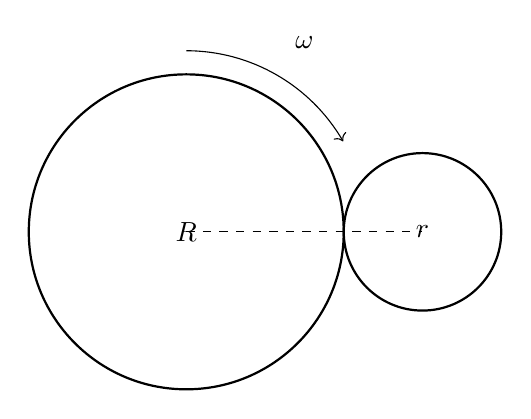
\begin{tikzpicture}[scale=1]

% Large disc
\draw[thick] (0,0) circle (2);
\node at (0,0) {$R$};


% Small disc
\draw[thick] (3,0) circle (1);
\node at (3,0) {$r$};

% Centers line
\draw[dashed] (0,0) -- (3,0);



% Angular velocity arrow
\draw[->] (0,2.3) arc (90:30:2.3);
\node at (1.5,2.4) {$\omega$};

\end{tikzpicture}
\end{center}

A) \(\dfrac{R+r}{r}\omega\)\\

B) \(\dfrac{R}{r}\omega\)\\

C) \(\dfrac{R}{R+r}\omega\)\\

D) \(\dfrac{r}{R}\omega\)

\item A particle executes SHM with amplitude \(A\) and angular frequency \(\omega\). At displacement \(x=\dfrac{A}{2}\), the spring constant is suddenly increased by factor \(1+\varepsilon\) while instantaneous velocity remains unchanged. Using conservation of total mechanical energy across the sudden change, determine the new amplitude correct to first order in \(\varepsilon\).\\

A) \(A\left(1-\dfrac{\varepsilon}{4}\right)\)\\

B) \(A\left(1-\dfrac{\varepsilon}{8}\right)\)\\

C) \(A\left(1-\dfrac{\varepsilon}{2}\right)\)\\

D) \(A\left(1+\dfrac{\varepsilon}{4}\right)\)

\item The gravitational field inside a hollow spherical shell is zero at all interior points; if a small mass is placed slightly off-center, the net force remains zero because vector contributions cancel even though gravitational potential is spatially constant throughout the interior region.\\

A) Exact symmetry cancellation\\

B) Zero enclosed mass\\

C) Inverse-square law alone\\

D) Linear force law

\item A rigid wheel rolls without slipping with translational acceleration \(a\) and angular acceleration \(\alpha\). Considering instantaneous kinematics of rim points relative to ground, identify instantaneous axis of rotation and its acceleration relative to ground.\\

A) Contact point, zero acceleration\\

B) Contact point, non-zero acceleration\\

C) Center, zero acceleration\\

D) Infinity, zero acceleration

\item In SHM, amplitude increases by \(10\%\) while spring constant decreases by \(10\%\); retaining second-order terms in small quantity \(0.1\), determine percentage change in total mechanical energy \(E=\frac{1}{2}kA^2\).\\

A) \(0\%\)\\

B) \(1\%\)\\

C) \(2\%\)\\

D) \(10\%\)

\item The free surface of a rotating liquid is given by \(z=\dfrac{\omega^2 r^2}{2g}\). If angular speed is increased by small fraction \(\varepsilon\), determine fractional increase in total gravitational potential energy of the liquid column retaining first-order terms.\\

A) \(2\varepsilon\)\\

B) \(\varepsilon\)\\

C) \(4\varepsilon\)\\

D) \(\dfrac{\varepsilon}{2}\)

\item Two waves of equal amplitudes and frequencies \(f\) and \(f+\Delta f\) interfere producing beats. If one source approaches observer with speed \(u\ll v\) where \(v\) is wave speed, determine beat frequency to first order in \(u/v\).\\

A) \(\left|\Delta f+\dfrac{fu}{v}\right|\)\\

B) \(\left|\Delta f-\dfrac{fu}{v}\right|\)\\

C) \(|\Delta f|\)\\

D) \(\left|2\Delta f\right|\)

\end{enumerate}

\end{document}